% !TeX spellcheck = en_US
% !TeX root = ../build/aggregator.tex
% !TeX TXS-program:compile = txs:///xelatex/[--shell-escape]



%%%%%%%%%%%%%%%%%%%%%%%%%%%%%%%%%%%%%%%%%%%%%%%%%%%%%%%%%%%%%%%%%%%%%%%%%%
\section{Introduction}


In this document, we delve into a crucial component of the zkEVM called the
\textbf{Aggregator}. Informally speaking, the \textbf{Aggregator} is in charge of gluing several proofs stating batch correct execution into a single one. This glued proof ensures that if it is correct, then all the individual proofs for each batch are also accurate. The mechanisms used by the \textbf{Aggregator} in order to generate such a aggregated proof are known as \textbf{proof recursion} and \textbf{proof aggregation}. This approach of aggregating proofs aims to increase the throughput of the system. We will give some insights on how both mechanisms work.

In this document, we will also discuss topics such as the \textit{``prove anything'' paradigm}, a mechanism that allows the proof of any input, regardless of whether it is erroneous. In the case of an invalid input, instead of proving a state change, a no state change will be proven. We will also explore \textbf{zkCounters}, which are a mechanism we use to prevent our batch from fitting into the available execution traces in the system. In the event of exceeding such length limits, an out of counters (OCC) error will occur. To conclude, we will discuss how to eliminate zkCounters in the future by implementing a method known as Variable Degree Composite
Proofs (VADCOPs).





%%%%%%%%%%%%%%%%%%%%%%%%%%%%%%%%%%%%%%%%%%%%%%%%%%%%%%%%%%%%%%%%%%%%%%%%%
\section{``Prove Anything'' Paradigm}

To address the potential threat of \textbf{byzantine} (i.e., malicious) \textbf{sequencers}, we adhere to the ``prove anything' ' paradigm. Under this approach, the prover possesses the capability to generate a proof of execution for any input data. The only condition is that the batch must maintain a bounded amount of data, a requirement enforced by the smart contract during the sequencing process. The batch execution is carried out for any input data, resulting in the generation of a proof that either confirms a \textbf{state change} for correct input data or \textbf{no state change} for wrong input data, as we can observe in Figure \ref{fig:prove-anything}. This strategy ensures robust validation of the execution outcomes, providing a reliable mechanism to handle potential malicious behavior.

\begin{figure}[H]
\centering
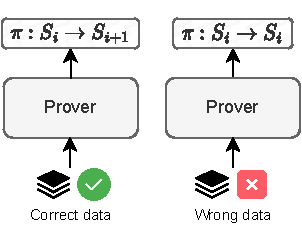
\includegraphics[width=0.4 \textwidth]{\zkevmdir/figures/architecture/aggregator/prove-anything.drawio}
\caption{The ``Prove Anything'' paradigm: If the data is correct the state change, but if it is not correct, the state does not change. The proof will respect both circumstances. }
\label{fig:prove-anything}
\end{figure}

\paragraph*{Invalid Transactions} Below we describe some errors in transactions that will cause the state to remain unchanged, as shown in Figure \ref{fig:invalid-txs}.

\begin{itemize}

\item \textbf{Reverted transaction}:
A transaction may revert during execution due to many reasons such as running out of gas, having a stack that is too large, or encountering a revert call in the code. This is a common scenario in EVM processing.

\item \textbf{Invalid intrinsic transaction}:
It is a transaction that is unable to be processed and has no impact on the current state. Keep in mind that this transaction could be part of a virtual batch. Example of errors in this scenario are: incorrect nonce, insufficient balance, etc. Our trusted sequencer is unlikely to input an incorrect nonce. However, any member of the community can submit a batch, which may result in an error.

\end{itemize}

\begin{figure}[H]
\centering
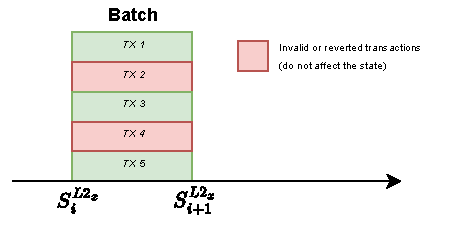
\includegraphics[scale=0.9]{\zkevmdir/figures/architecture/aggregator/proof-invalid-txs.drawio}
\caption{Invalid and reversed transactions have no impact on the state when the batch is executed.}
\label{fig:invalid-txs}
\end{figure}

\paragraph*{Invalid Batches} Errors might also occur at the batch level. Below we describe some errors in batches that will cause the state to remain unchanged, as shown in Figure \ref{fig:invalid-batch}.


\begin{itemize}
\item \textbf{Invalid Data.}
We are unable to decode (RLP-encoded) transactions , so we have \textbf{garbage input}.

\item \textbf{Prover resources exhaustion.}
The zkEVM manages this via row counters, also known as \textbf{zkCounters}. The batch cannot be processed due running of row counters.
\end{itemize}

\begin{figure}[H]
\centering
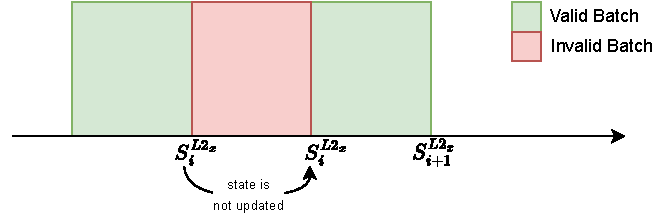
\includegraphics[scale=0.8]{\zkevmdir/figures/architecture/aggregator/proof-invalid-batch.drawio}
\caption{If a batch is invalid, the state remains unchanged.}
\label{fig:invalid-batch}
\end{figure}

Figure \ref{fig:invalid-batch} shows that when a batch processing fails, the state remains unchanged $S_{i+1}=S_i$ and a proof of this lack of state change is produced. This occurrence should be infrequent yet it is possible.

The \textit{prove anything} approach allows us to implement an anti-censorship measure called \textbf{forced batches}. Using these approach, a user can take the role of a sequencer for getting its L2 transactions into the virtual state in case the trusted sequencer is not doing so. The main use case is to allow a user to send bridge transactions in order to withdraw assets from L2 without the risk of censorship (which will make it impossible to withdraw the funds). Since it is an (untrusted) user who is sending the L2 batch data, we must be sure that we can prove anything that the user sends. The forced batches mechanism will be explained later on (when describing the different security measures implemented in the zkEVM).



%%%%%%%%%%%%%%%%%%%%%%%%%%%%%%%%%%%%%%%%%%%%%%%%%%%%%%%%%%%%%%%%%%%%%%
\section{zkCounters}

After addressing counters before, it is crucial to highlight their significance. Counters are used to monitor the row count in each State Machine, including the Main SM, during the execution of a particular batch.

The management of these counters is incorporated inside the computation process. By doing so, when the computation uses up all its assigned resources while generating the proof, the system is able to proof that a batch does not cause a change in the state. This issue is referred to as a \textbf{Out Of Counters (OOC) error}. This error is very specific to our zkEVM State Machine-like design, because of having fixed number of rows. Figure \ref{fig:ooc-error} shows an out of counters situation.

Although at the present there exists this backend limitation in the proving system that forces execution traces for all the States Machines to have the same amount of rows, it is expected to be removed with the forthcoming introduction of \textbf{VADCOPs: Variable Degree Composite Proofs}. Currently in development, VADCOPs will provide the capability to partition a large State Machine, originally comprising a high amount of rows, into smaller execution traces with fewer rows. This will offer several advantages, with the most notable one being the elimination of zkCounters for prover's resource management. The main idea for VADCOPs is depicted in Figure \ref{fig:vadcops}. The ongoing development of VADCOPs includes a rewriting of both the cryptographic backend and the constraint language, which will be called PIL2.


\begin{figure}[h]
\centering
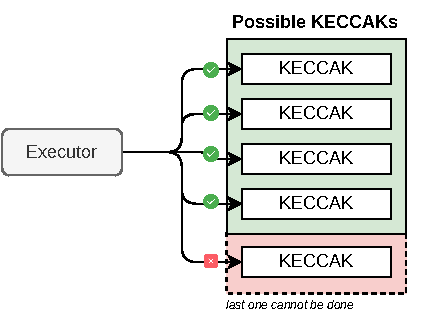
\includegraphics[scale=0.8]{\zkevmdir/figures/architecture/aggregator/zkcounters.drawio}
\caption{Out of counters error. Consider a scenario where our Keccak arithmetization permits only up to $4$ Keccak operations before exhausting the available rows. An out of counters error will occur if the transaction involves invoking $5$ (or more) Keccaks.
}
\label{fig:ooc-error}
\end{figure}

\begin{figure}[h]
\centering
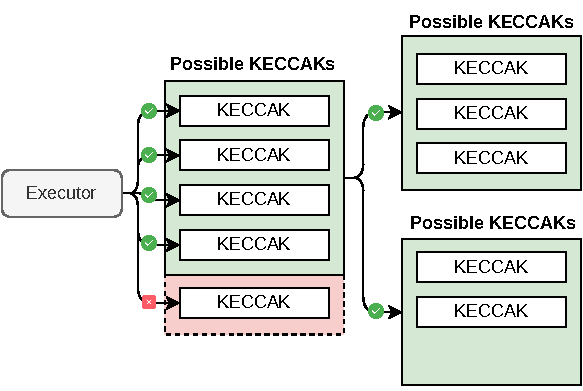
\includegraphics[scale=0.8]{\zkevmdir/figures/architecture/aggregator/vadcops.drawio}
\caption{Example of VADCOPs with KECCAKs. In this scenario, it becomes feasible to execute 5 Keccak operations despite the limit being 4 due to the State Machine's length. At a high level, the solution involves splitting the proof into two parts, each containing fewer rows, and then aggregating them to demonstrate the execution of $5$ Keccak operations.}
\label{fig:vadcops}
\end{figure}






%%%%%%%%%%%%%%%%%%%%%%%%%%%%%%%%%%%%%%%%%%%%%%%%%%%%%%%%%%%%%%%%%%%%%%%%%%
\section{Discussing the Proof}

The preceding section introduced VADCOPs. The concept of VADCOPs suggests that we can somehow aggregate proofs together. This allows verification to be performed only once, albeit with more effort on the prover's part. However, this scenario is of interest to us as it enables the aggregation of multiple proofs for different batches, creating a single unified proof that enables the verification of various batches simultaneously, ensuring the correct execution of all of them at once, incrementing the throughput of the system. There are two interesting techniques in this direction: \textbf{proof recursion} and \textbf{proof aggregation}.

\subsection{Proof Recursion}

\textbf{Recursion} (also called \textbf{compression}) in proof systems enables the prover to transition from large, time-consuming proofs to smaller, quicker-to-verify proofs. Essentially, the prover of the next stage proofs that the verification of the previous stage is correctly performed. In general, by the succinctness property of SNARKs, this makes the final proofs smaller and faster to verify. Notice that we can also change the set of public values from one stage to the next one. The diagram shown in Figure \ref{fig:proof-recursion} illustrates the core principle of proof recursion. This graphic representation highlights the efficiency improvements obtained through proof recursion, where each next proof is optimized in size compared to the previous one.

\begin{figure}[H]
\centering
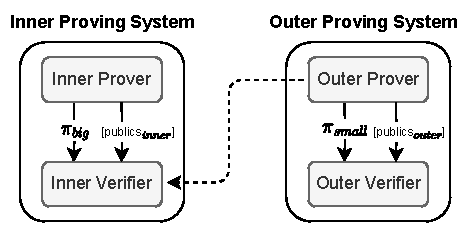
\includegraphics[scale=0.9]{\zkevmdir/figures/architecture/aggregator/proof-composition.drawio}
\caption{Illustration of Proof Recursion. The Outer Prover is responsible for proving the correct verification of the proof $\pi_{big}$, reducing the size of the proof due to the succinctness property of SNARKs, which dictates that the verification time should way less than the proving time.}
\label{fig:proof-recursion}
\end{figure}




\subsection{Proof Aggregation}

In the context of zkEVM, \textbf{Aggregation} is a technique that allows the prover to generate a single proof that covers multiple L2 batches. This reduces the number of proofs to verify, increasing the throughput of the system. With proof aggregation, we can send a single L1 transaction that aggregates multiple batches, improving the batch consolidation rate. The proving system restricts aggregation to only consecutive batches. Notice that we can aggregate proofs that prove a single batch with other that prove multiple batches, as shown in Figure \ref{fig:proof-aggregation}, thanks to a technique in the cryptographic backend that we call \textbf{normalization}. Finally, remark that the smart contract also limits the maximum number of batches that can be aggregated.

\begin{figure}[H]
\centering
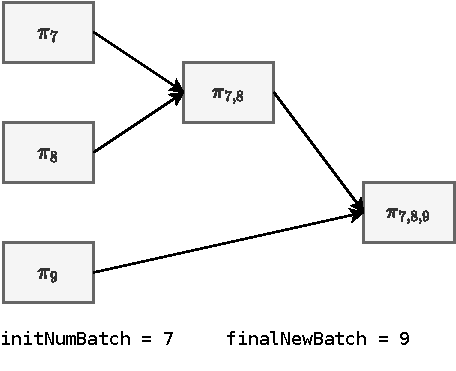
\includegraphics[scale=0.8]{\zkevmdir/figures/architecture/aggregator/recursion-aggregation-proof}
\caption{Proof Aggregation.}
\label{fig:proof-aggregation}
\end{figure}




\subsection{zkEVM Recursion and Aggregation}

In this section, we provide the concrete blocks and steps used to
prove the correct execution of a several batches by our zkEVM using recursion and aggregation. An overview of the overall process can be observed in Figure \ref{fig:zkevm-recursion}.


\begin{figure}[H]
\centering
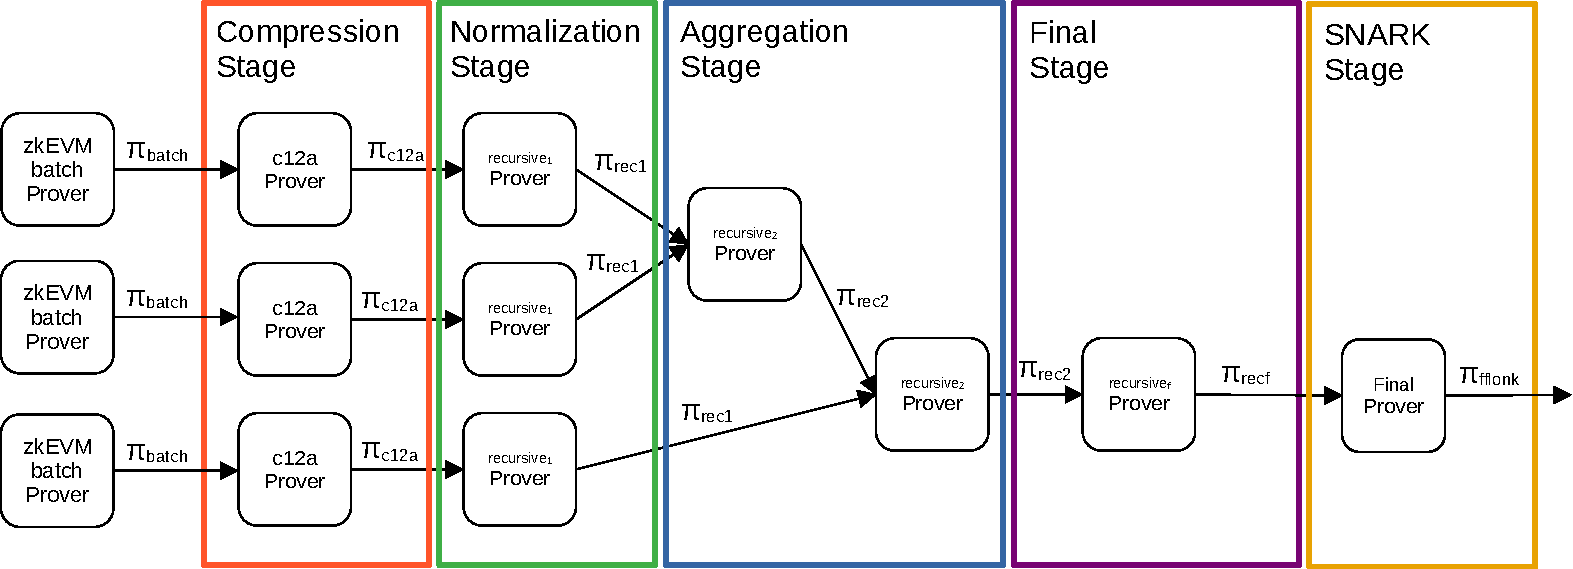
\includegraphics[width=0.9 \textwidth]{\zkevmdir/figures/architecture/aggregator/recursive-diagram}
\caption{zkEVM specific recursion design diagram.}
\label{fig:zkevm-recursion}
\end{figure}


The first proving system generates such a big proof since it has a lot of high degree polynomials. Henceforth, a first \textit{Compression Stage} its invoked in each batch's proof, aiming to reduce the number of polynomials used, allowing to reduce the proof size.

Once the compression step has been completed, a proof aggregation stage will be in charge of joining several batches proofs into a single proof proving each of the single proofs all at once. The way of proceeding will be to construct a binary tree of proofs by aggregating two by two each of them. We will call this the \textit{Aggregation Stage}.

Next, a \textit{Normalization Stage} is invoked, allowing each aggregator verifiers and the normalization verifiers to be exactly the same, permitting successful aggregation via a recursion.

Once the normalization step has been finished, its time for aggregation. In this step we are going to join two batches' proofs together, which will be done many times until only one proof spares. Observe that the \textit{Aggregation Stage} needs to be designed in order to accept either already aggregated proofs or only compressed ones.

The \textit{Final Stage} is the very last STARK step among the recursion process, which is in charge of verifying a proof over a completely different finite field, the one defined by the \texttt{bn128} elliptic curve. This is done in this way because, in the next step of the process, a SNARK Groth16 proof, which works over elliptic curves, will be generated.



%%%%%%%%%%%%%%%%%%%%%%%%%%%%%%%%%%%%%%%%%%%%%%%%%%%%%%%%%%%%%%%%%
\section{Introducing the Aggregator}

The \textbf{aggregator} is the component within the zkEVM architecture that will be in charge of performing the proof aggregation schema. The aggregator invokes the \texttt{verifyBatches()} function (See Figure \ref{fig:aggregator}) on the smart contract, passing parameters such as the initial batch number \texttt{initNumBatch}, the final batch number (\texttt{finalNewBatch}), the \texttt{newStateRoot}, and the aggregated proof $\pi$. The previous root is stored in the smart contract, eliminating the need to transmit it. Recall that the smart contract contains a summary of the batch information in the accumulated input hash.


\begin{figure}[h]
\centering
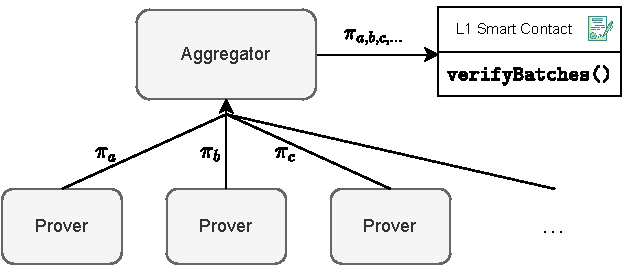
\includegraphics[width=0.6\textwidth]{\zkevmdir/figures/architecture/aggregator/aggregator.drawio}
\caption{The role of the Aggregator is to aggregate several proofs in one and send it to the L1 Smart Contract through the \texttt{verifyBatches()} function.}
\label{fig:aggregator}
\end{figure}

The aggregator operates as a network server, establishing connections with provers that function as network clients. Provers link up with the aggregator to send their proofs. The aggregator, acting as a server, is responsible for deciding how to horizontally scale provers in order to achieve an optimal batch consolidation rate. Scaling is essential to avoid an accumulation of extra batches awaiting consolidation. The aggregator keeps a record of authorized provers. Both the aggregator and the provers operate in a cloud-based environment (See Figure \ref{fig:aggregator-cloud}), with the provers being configured as high-resource instances. This configuration enables effective and scalable control of evidence processing, guaranteeing the system can handle different workloads and maintain an efficient batch consolidation rate.


\begin{figure}[h]
\centering
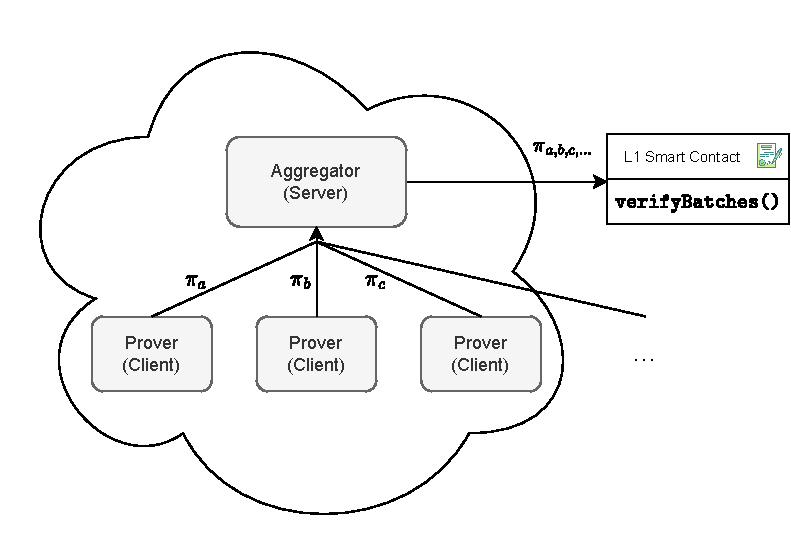
\includegraphics[width=0.6\textwidth]{\zkevmdir/figures/architecture/aggregator/aggregator-cloud.drawio}
\caption{The aggregator role depicted in a cloud-based enviroment.}
\label{fig:aggregator-cloud}
\end{figure}



%%%%%%%%%%%%%%%%%%%%%%%%%%%%%%%%%%%%%%%%%%%%%%%%%%%%%%%%%%%%%%%%%
\subsection{Inputs and Outputs of the Proof}

The proof generation process requires several inputs, as shown in Figure \ref{fig:aggregator-only-publics}, to ensure its soundness:

\begin{itemize}

\item The \textbf{aggregator address}, serving as a safeguard against malleability in the \texttt{verifyBatches()} function, ensuring that no one can use another aggregator's proof.

\item The previous state root (\texttt{oldStateRoot}), which is already included in the smart contract and does not require explicit sending.

\item The previous accumulated input hash (\texttt{oldAccInputHash}).

\item The initial batch number (\texttt{initNumBatch}).

\item The \texttt{chainID} and the \texttt{forkID} ensure that the proof is valid only within the intended chain and version of the zkEVM.


\end{itemize}


The aggregator generates three outputs: the updated state root (\texttt{newStateRoot}), the new accumulated input hash (\texttt{newAccInputHash}) and the batch number of the last batch included in the the aggregated proof once it has been successfully generated (\texttt{finalNewBatch}). At the moment all the inputs and outputs are public, presenting an efficiency problem as we will see below.


\begin{figure}[h]
\centering
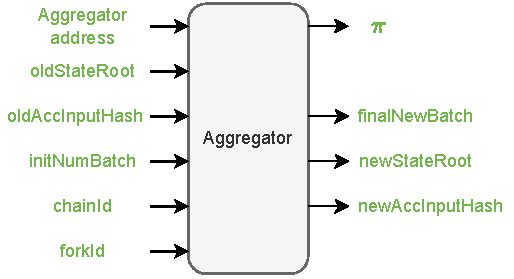
\includegraphics[scale=0.8]{\zkevmdir/figures/architecture/aggregator/aggregator-design-only-publics.drawio}
\caption{Public inputs are shown in green, whereas private inputs are shown in red for distinction. The diagram shows the inputs of the aggregator, all of which are, at this moment, publicly available. }
\label{fig:aggregator-only-publics}
\end{figure}


The smart contract structure shown in Figure \ref{fig:verifier-smart-contract} enables the ability to upgrade or alter the verifier as necessary. Currently we only provide a verifier called \href{https://github.com/0xPolygonHermez/zkevm-contracts/blob/main/contracts/verifiers/FflonkVerifier.sol}{\texttt{FflonkVerifier.sol}}.

\begin{figure}[h]
\centering
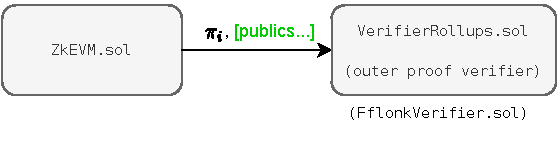
\includegraphics[scale=0.8]{\zkevmdir/figures/architecture/aggregator/verifier-contract.drawio}
\caption{Verifier Contract redesign.}
\label{fig:verifier-smart-contract}
\end{figure}


With this approach, the verifier must utilize a list of publics. However, a verifier with a single input is more cost-effective. In Groth16, there is a scalar multiplication operation per public input, which is approximately $10,000$ Gas per public. The key is to create a single public input that is the hash of all the previous public keys and then transform these public inputs into private inputs, as shown in Figure \ref{fig:aggregator-with-privates}. Henceforth, for the \textbf{outer proof}, there will be a single public input in the aggregator called \texttt{inputSnark}. This is a KECCAK hash of all the previous public inputs and outputs.


\begin{figure}[h]
\centering
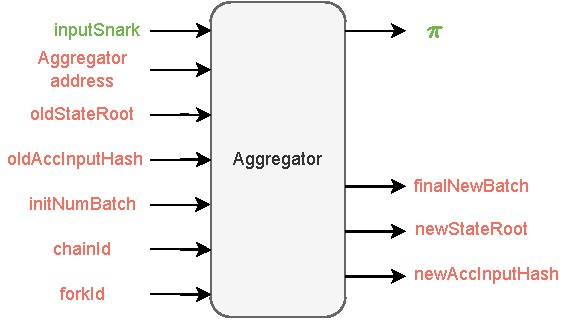
\includegraphics[scale=0.8]{\zkevmdir/figures/architecture/aggregator/aggregator-design-with-privates.drawio}
\caption{Aggregator with privates. The \texttt{inputSnark} parameter is the has of all our previous public inputs and outputs. Observe that this parameter is the only public parameter of the aggregator, altogether with the proof. }
\label{fig:aggregator-with-privates}
\end{figure}


As shown in Figure \ref{fig:verifier-smart-contract-redesign}, when \texttt{zkEVM.sol} interacts with the \texttt{VerifierRollups.sol} smart contract in the revised procedure, only a single public parameter is passed, which helps in minimizing data transmission expenses. This optimized approach requires two crucial verifications by the proof system. Initially, it verifies that the hash of all private inputs, arranged in the correct order, corresponds to the given \texttt{inputSnark}. The proof system verifies that the total input hash calculated for all processed batches by the aggregator matches the specified \texttt{newAccInputHash}.


\begin{figure}[h]
\centering
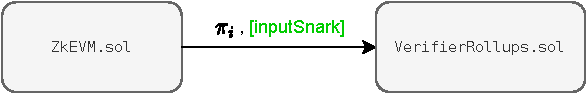
\includegraphics[scale=0.8]{\zkevmdir/figures/architecture/aggregator/verifier-contract-redesign.drawio}
\caption{Verifier Contract redesign.}
\label{fig:verifier-smart-contract-redesign}
\end{figure}
